\section{Adding Prudence to Process}
Fortunately, the risk of negligence liability and the cost to defend
unavoidable risks can be reduced. This research includes an analysis of safety
critical software systems that identifies the specific inequities of software
that complicate process interpretation. We then determine the inadequacies of
current practices that increase the risk of negligence liability in software.
We finally provide recommendations to enhance an organization�s process and
mitigate this risk.

Our solution aims to minimize risks in safety-critical software environments and
reduce the cost to defend negligence liabilities in the case of legal disputes.
The documentation process is the key to our solution. Documentation is an
effective way to find bugs in a software program and thoroughly testing it may
be the most cost-effective way to reduce the risk of legal disputes
\cite{Kaner_doc_1995}. The model proposed in this paper introduces an
improvement to the software engineering workflow designed for safety-critical
environments that will provide traceable documentation that developers can use
minimize software defects and lawyers can use to defend (or confirm) negligence.

\begin{figure}
\begin{itemize}
  \item \textbf{Constraints on system}
    \begin{itemize}
      \item allows easy, real-time commenting for developers
      \item integrates commenting capabilities into IDE
      \item indexes comments based on code references, author, version
    \end{itemize}
  \item \textbf{Constraints on data representation}
    \begin{itemize}
      \item stores documentation comments in separate from code
      \item associates comment-to-code with a many-to-many relationship
      \item stores comment versioning and ownership information
      \item preserves comment-to-code associations through code changes
    \end{itemize}
\end{itemize}
\caption{Design goals for the system}
\label{design_criteria}
\end{figure}

\subsection{Comment Classification}
A \textbf{software comment} is a fragment of natural language intended for human
consumption. More formally, a comment is ``\textit{explanatory text embedded in
program source intended to help human readers understand it."} \cite{FOLDOC}.
For the purposes of this research, comments can be distinguished into two
different classes: 
\begin{enumerate}
  \item code comments
  \item documentation comments
\end{enumerate}

\textbf{Code comments} refer to the in-line comments that programmers write to
describe specific behavior of small snippets of code. In Java or C, these types
of comments are normally preceded by \verb!//! or surrounded by \verb!/*! and
\verb!*/!. \textbf{Documentation comments} refer to comments used as reference
material intended for human consumption to describe larger areas of code or
entire functions. Javadoc \cite{Javadoc} is a popoular representation of
documentation comments. They are distinguished by a preceding \verb!/**! and a
trailing \verb!*/!.

\subsection{Data Representation}

\begin{figure}
\begin{narrow}{-1.5in}{-1.5in}
\begin{center}
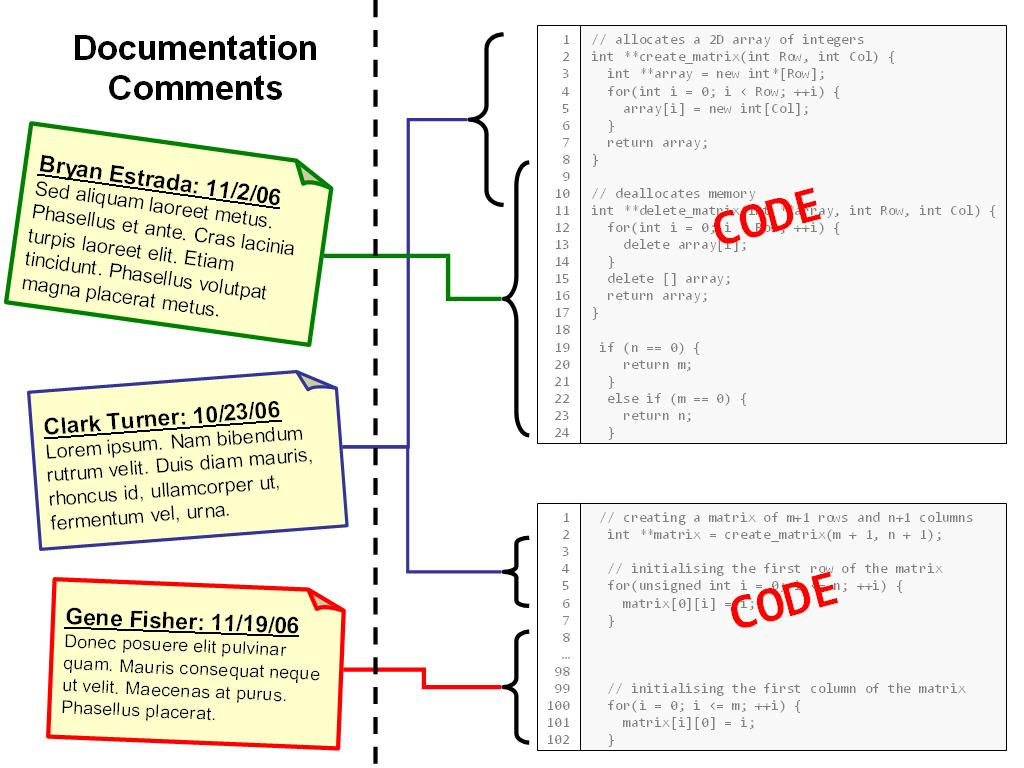
\includegraphics[scale=0.66]{images/comments.jpg}
\end{center}
\end{narrow}
\caption{Overview of comment-to-code association}
\label{comment_to_code}
\end{figure}

\subsection{Data Access}
\subsubsection*{Setting Data}
\subsubsection*{Retrieving Information}

